\documentclass{beamer}
\usetheme{Hannover}

\usepackage{sansmathaccent}
\pdfmapfile{+sansmathaccent.map}

\usepackage{bookmark}
\usepackage{subcaption}

\usepackage[ruled]{algorithm2e}
\SetKwInput{KwInput}{Input}                
\SetKwInput{KwOutput}{Output} 

\usepackage{tikz}
\usetikzlibrary{backgrounds, arrows.meta, shapes.geometric,
decorations.pathreplacing, calligraphy,
positioning }
\tikzset{%
>={Latex[width=2mm,length=2mm]},
  % Specifications for style of nodes:
            base/.style = {circle, draw=black,
                            fill=blue!30, minimum width=0.5cm, minimum
                            height=0.5cm, font=\sffamily\tiny,},
                            label/.style = {circle, draw=white, fill=white,
                            font=\sffamily\normalsize, opacity=0, text opacity=1}
}

\title{Planar Graphs}
\subtitle{and how to find them}
\author{Brendan Halstead}
\date{July 21, 2020}

\begin{document}
    \frame{\titlepage} % # 1
    \section[Outline]{}
    \frame{\tableofcontents}

    \section{Definitions and Examples}
        \frame % # 2
        {
            \frametitle{What is a planar graph?}
            \textbf{Planar embedding}: drawing of a graph with no edges crossing
            \medskip
            \textbf{Planar graph}: has a planar embedding

            \bigskip
            \pause
            
            \begin{figure}[h!]
                \centering
                \begin{subfigure}[b]{0.4\textwidth}
                    \centering
                    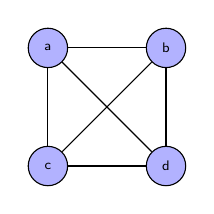
\begin{tikzpicture}[node distance=1.5cm, every node/.style={base}, align=center, tight background]
                        \node (1){ a};
                        \node (2)[right of=1]{b};
                        \node (3)[below of=1]{c};
                        \node (4)[below of=2]{d};
                        \draw (1)--(2);
                        \draw (2)--(3);
                        \draw (3)--(4);
                        \draw (4)--(1);
                        \draw (1)--(3);
                        \draw (2)--(4);
                    \end{tikzpicture}
                    \subcaption*{Nonplanar embedding}
                \end{subfigure}
                \pause
                \begin{subfigure}[b]{0.4\textwidth}
                    \centering
                    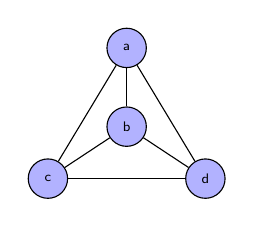
\begin{tikzpicture}[node distance=1cm, every node/.style={base}, align=center, tight background]
                        \node (1){a};
                        \node (2)[below of=1]{b};
                        \node (3)[left of=2, yshift=-0.66cm]{c};
                        \node (4)[right of=2, yshift=-0.66cm]{d};
                        \draw (1)--(2);
                        \draw (2) -- (3);
                        \draw (3)--(4);
                        \draw (4)--(1);
                        \draw (1)--(3);
                        \draw (2)--(4);
                    \end{tikzpicture}
                    \subcaption*{Planar embedding}
                \end{subfigure}  
            \end{figure}

            \pause
            \medskip

            $K_4$ is planar!
         
        }
    
        \frame % # 2
        {
            \frametitle{Another example}
            The complete bipartite graph $K_{3,3}$
            \medskip
            \begin{figure}[h]{}
                \centering
                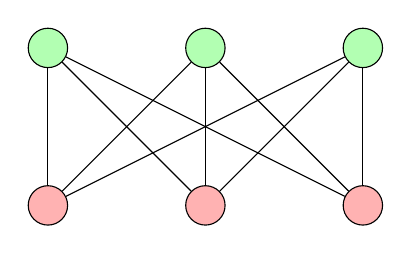
\begin{tikzpicture}[node distance=2cm, every node/.style={base}, align=center, tight background]
                    \node[fill=green!30] (1) {};
                    \node[right of=1, fill=green!30] (2){};
                    \node[right of=2, fill=green!30](3){};
                    \node[below of=1, fill=red!30] (4){};
                    \node[below of=2, fill=red!30] (5){};
                    \node[below of=3, fill=red!30] (6){};
                    \pause
                    \draw (1)--(4);
                    \draw (1)--(5);
                    \draw (1)--(6);
                    \draw (2)--(4);
                    \draw (2)--(5);
                    \draw (2)--(6);
                    \draw (3)--(4);
                    \draw (3)--(5);
                    \draw (3)--(6);
                \end{tikzpicture}
            \end{figure}  

            \pause
            \onslide<2-> {$K_{3,3}$ is \textbf{not} planar.}

        }


    \section{Kuratowski's Theorem}
    
        \frame % 3
        {
            \frametitle{Kuratowski's Theorem}
            
            \textbf{Theorem:} A graph is planar if and only if it contains no subgraphs
            homeomorphic to $K_{5}$ or $K_{3,3}$.
            
            \bigskip
            
            \begin{figure}[h!]
                \centering
                \begin{subfigure}[b]{0.4\textwidth}
                    \centering
                    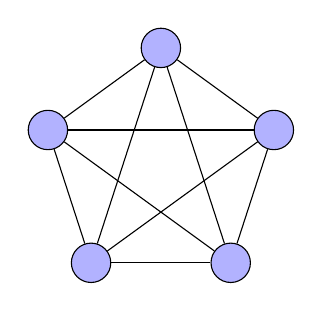
\begin{tikzpicture}[ node distance=1cm, every node/.style={base}, align=center, tight background]
                        \def\ngon{5}
                        \node[color=white, regular polygon,regular polygon sides=\ngon,minimum size=3cm] (p) {};
                        \foreach\x in {1,...,\ngon}{\node (p\x) at (p.corner \x){};}
                        \foreach\x in {1,...,\numexpr\ngon-1\relax}{
                            \foreach\y in {\x,...,\ngon}{
                                \draw (p\x) -- (p\y);
                            }
                        }
                    \end{tikzpicture}
                    \subcaption*{$K_5$}
                \end{subfigure}
                \begin{subfigure}[b]{0.5\textwidth}
                    \centering
                    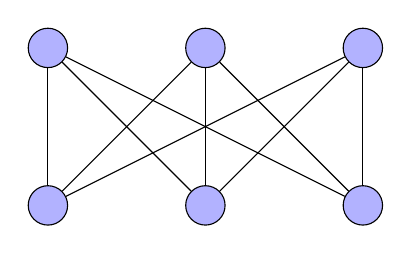
\begin{tikzpicture}[node distance=2cm, every node/.style={base}, align=center, tight background]
                        \node (1){};
                        \node (2)[right of=1]{};
                        \node (3)[right of=2]{};
                        \node (4)[below of=1]{};
                        \node (5)[below of=2]{};
                        \node (6)[below of=3]{};
                        \draw (1)--(4);
                        \draw (1)--(5);
                        \draw (1)--(6);
                        \draw (2)--(4);
                        \draw (2)--(5);
                        \draw (2)--(6);
                        \draw (3)--(4);
                        \draw (3)--(5);
                        \draw (3)--(6);
                    \end{tikzpicture}
                    \subcaption*{$K_{3,3}$}
                \end{subfigure}
                  
            \end{figure}
            Homeomorphic to = has same basic shape as
        
        \vfill   

        }

        \frame % # 2
        {
            \frametitle{Example}
            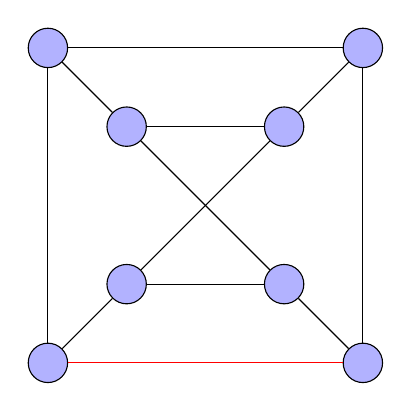
\begin{tikzpicture}[ node distance=2cm, every node/.style={base}, align=center, tight background]
                \node (p1) at (1,0){};
                \node[right of=p1] (p2){};
                \node[below of=p2] (p3){};
                \node[left of=p3] (p4){};
                \tikzset{node distance = 4cm}
                \node (p5) at (0,1){};
                \node[right of=p5] (p6){};
                \node[below of=p6] (p7){};
                \node[left of=p7] (p8){};
                \draw (p5) -- (p6);
                \draw (p5) -- (p8);
                \draw (p5) --(p1);
                \draw (p6) -- (p2);
                \draw (p6) -- (p7);
                \draw (p7) -- (p3);
                \draw (p7) -- (p8);
                \draw (p8) -- (p4);

                \draw (p1) -- (p2);
                \draw (p3) -- (p4);
                \draw (p1) -- (p3);
                \draw (p2) -- (p4);
                \pause
                \draw[red] (p7) -- (p8);
                % \tikzset{node distance = 0cm}
                % \node[above of=p1, fill=red!30](p1red) {};
                % \node[above of=p2, fill=red!30](p2red) {};
                % \node[above of=p3, fill=red!30](p3red) {};
                % \node[above of=p3, fill=red!30](p3red) {};
                % \node[above of=p3, fill=red!30](p3red) {};
                % \node[above of=p3, fill=red!30](p3red) {};
                % \node[above of=p3, fill=red!30](p3red) {};
            \end{tikzpicture} 
            
        }
        \frame % # 2
        {
            \frametitle{Example}
            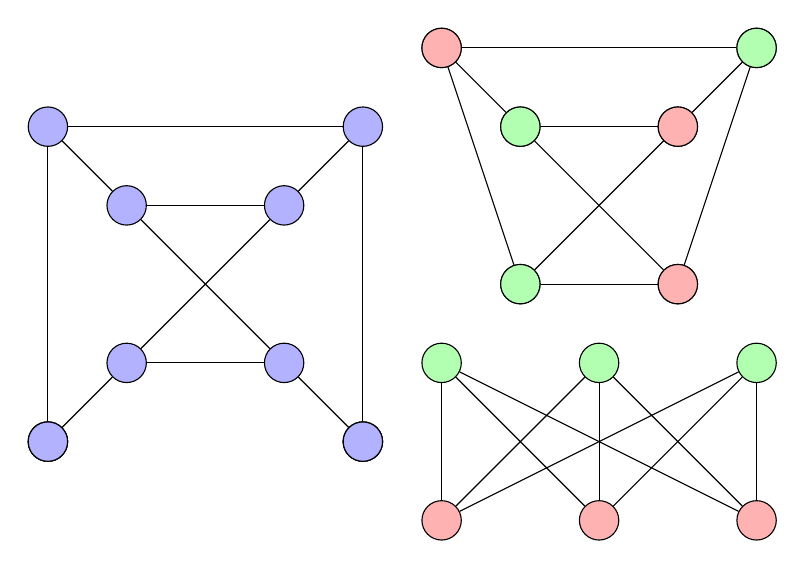
\begin{tikzpicture}[ node distance=2cm, every node/.style={base}, align=center, tight background]
                \node (p1) at (1,0){};
                \node[right of=p1] (p2){};
                \node[below of=p2] (p3){};
                \node[left of=p3] (p4){};
                \tikzset{node distance = 4cm}
                \node (p5) at (0,1){};
                \node[right of=p5] (p6){};
                \node[below of=p6] (p7){};
                \node[left of=p7] (p8){};
                \draw (p5) -- (p6);
                \draw (p5) -- (p8);
                \draw (p5) --(p1);
                \draw (p6) -- (p2);
                \draw (p6) -- (p7);
                \draw (p7) -- (p3);
                \draw (p8) -- (p4);

                \draw (p1) -- (p2);
                \draw (p3) -- (p4);
                \draw (p1) -- (p3);
                \draw (p2) -- (p4);

                \pause
                \tikzset{node distance = 0cm}
                \node[above of=p8, fill=red!30] (p8color) {};
                \node[above of=p7, fill=red!30] (p7color) {};

                \pause
                \node[above of=p8color] (p8blue) {};
                \node[above of=p7color] (p7blue) {};
                \tikzset{node distance = 2cm}
                \node (h1) at (6,1){};
                \node[right of=h1] (h2){};
                \node[below of=h2] (h3){};
                \node[left of=h3] (h4){};
                \node (h5) at (5,2) {};
                \node (h6) at (9,2) {};

                \draw (h1) -- (h2);
                \draw (h3) -- (h4);
                \draw (h1) -- (h3);
                \draw (h2) -- (h4);
                \draw (h5) -- (h1);
                \draw (h5) -- (h4);
                \draw (h6) -- (h2);
                \draw (h6) -- (h3);
                \draw (h5) -- (h6);
                
                \pause
                \tikzset{node distance = 0cm}
                \node[above of=h1, fill=green!30] (h1color) {};
                \node[above of=h4, fill=green!30] (h4color) {};
                \node[above of=h6, fill=green!30] (h6color) {};
                \node[above of=h2, fill=red!30] (h2color) {};
                \node[above of=h3, fill=red!30] (h3color) {};
                \node[above of=h5, fill=red!30] (h5color) {};
            
                \pause
                \tikzset{node distance = 2cm}
                \node[fill=green!30] (1) at (5,-2){};
                \node[right of=1, fill=green!30] (2){};
                \node[right of=2, fill=green!30] (3){};
                \node[below of=1, fill=red!30] (4){};
                \node[below of=2, fill=red!30] (5){};
                \node[below of=3, fill=red!30] (6){};
                \draw (1)--(4);
                \draw (1)--(5);
                \draw (1)--(6);
                \draw (2)--(4);
                \draw (2)--(5);
                \draw (2)--(6);
                \draw (3)--(4);
                \draw (3)--(5);
                \draw (3)--(6);

                % \tikzset{node distance = 0cm}
                % \node[above of=p1, fill=red!30](p1red) {};
                % \node[above of=p2, fill=red!30](p2red) {};
                % \node[above of=p3, fill=red!30](p3red) {};
                % \node[above of=p3, fill=red!30](p3red) {};
                % \node[above of=p3, fill=red!30](p3red) {};
                % \node[above of=p3, fill=red!30](p3red) {};
                % \node[above of=p3, fill=red!30](p3red) {};
            \end{tikzpicture} 
            \vfill
        }
    \section{DMP Algorithm}

    

    \frame % 3
    {
        \frametitle{Background}
        Published by Demoucron, Malgrange and Pertuiset in 1964

        \bigskip
        Works by adding segments to a subgraph until graph is complete or segment is
        blocked

        \bigskip
        Not the most efficient, but simplest to understand

        \bigskip
        Requires pre-processing

        \vfill
    }
    
    \frame
    {
        \frametitle{DMP Planarity Algorithm}
        
        
        \begin{figure}
            \centering
            \SetCustomAlgoRuledWidth{5.5cm}
            \tiny
            \begin{subfigure}[h]{5.5cm} 
                \begin{algorithm}[H]
                    \NoCaptionOfAlgo
                    \DontPrintSemicolon
                    \KwInput{A 2-connected graph G}
                    \KwOutput{A planar embedding or FALSE}
                    $G_0$ := any cycle in G \;
                    
                    
                    \caption{\tiny DMP Algorithm}
                \end{algorithm} 
            \end{subfigure}
            
        \end{figure}
        \vfill
    }
    \frame % 3
    {
    
        \frametitle{DMP Planarity Algorithm}
        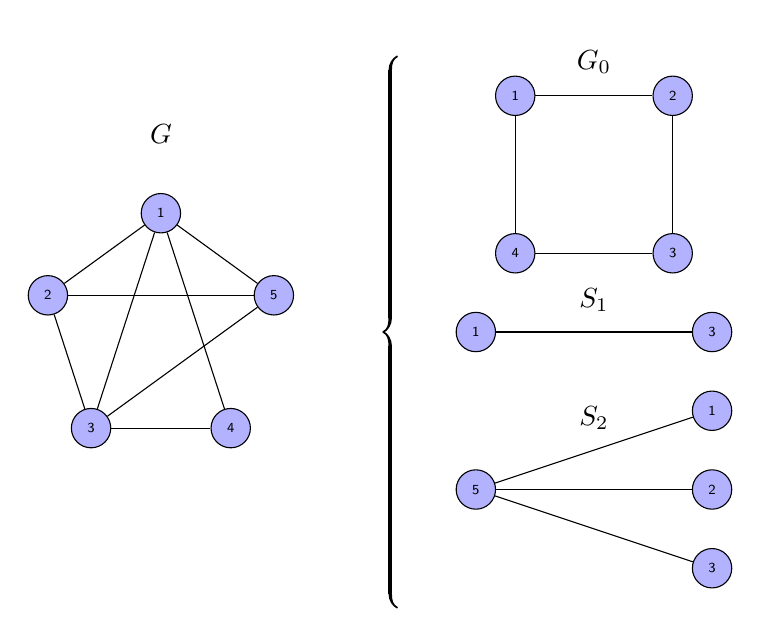
\begin{tikzpicture}[ node distance=1cm, every node/.style={base}, align=center, tight background]
            \def\ngon{5}
            \node[color=white, regular polygon,regular polygon sides=\ngon,minimum size=3cm] (p) {};
            \foreach\x in {1,...,\ngon}{\node (p\x) at (p.corner \x){\tiny \x};}
            \foreach\x in {1,...,\numexpr\ngon-2\relax}{
                \foreach\y in {\number\numexpr\x+1\relax}{\draw (p\x) -- (p\y);}
            }
            \draw (p1) -- (p3);
            \draw (p1) -- (p4);
            \draw (p1) --(p5);
            \draw (p2) -- (p5);
            \draw (p3) -- (p5);
            \pause
            
            \draw[decorate, decoration={calligraphic brace,amplitude=5pt}, line
            width=1.25pt] (3,-3.5) -- (3,3.5);
            \node[label, above of=p1]{$G$};

            \tikzset{node distance = 2cm}
            \node (g01) at (4.5,3) {1};
            \node[right of=g01] (g02)  {2};
            \node[below of=g02] (g03)  {3};
            \node[below of=g01] (g04)  {4};
            \draw (g01) -- (g02) node [label, midway, above] {$G_0$};
            \draw (g02) -- (g03);
            \draw (g03) -- (g04);
            \draw (g04) -- (g01);
            \pause

            \tikzset{node distance = 1cm}
            \node(s11) at (4,0){1};
            \node(s13) at (7,0){3};
            \draw (s11) -- (s13) node [label, midway, above] {$S_1$};

            \node[below of=s11, yshift=-1cm](s25) {5};
            \node[right of=s25, xshift=2cm](s22) {2};
            \node[above of=s22](s21) {1};
            \node[below of=s22](s23) {3};
            \draw (s25) -- (s21) node [label, midway, above] {$S_2$};
            \draw (s25) -- (s22);
            \draw (s25) -- (s23);

        \end{tikzpicture} 
    }
    
    \frame
    {
        \frametitle{DMP Planarity Algorithm}
        \begin{figure}
            \centering
            \SetCustomAlgoRuledWidth{5.5cm}
            \tiny
            \begin{subfigure}[h]{5.5cm} 
                \begin{algorithm}[H]
                    
                    \NoCaptionOfAlgo
                    \DontPrintSemicolon
                    \KwInput{A 2-connected graph G}
                    \KwOutput{A planar embedding or FALSE}
                    $G_0$ := any cycle in G \;
                    \While{$G_j \neq G$}
                        {
                            \If{any segment is blocked}
                            {
                                \Return FALSE \;
                            }
                        }
            
                    \caption{\tiny DMP Algorithm}
                \end{algorithm}
            \end{subfigure}
        \end{figure}
        \vfill
    }

    \frame 
    {
    
        \frametitle{DMP Planarity Algorithm}
        \centering
            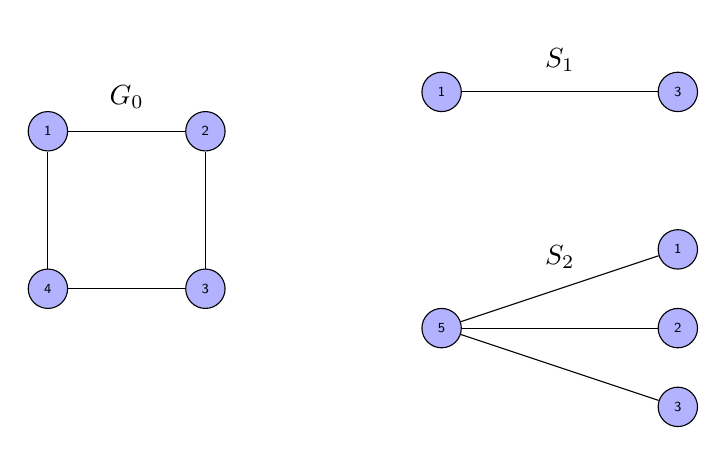
\begin{tikzpicture}[ node distance=1cm, every node/.style={base}, align=center, tight background]
                
                \tikzset{node distance = 2cm}
                \node (g01) at (-1,0.5){1};
                \node[right of=g01] (g02)  {2};
                \node[below of=g02] (g03)  {3};
                \node[below of=g01] (g04)  {4};
                \draw (g01) -- (g02) node [label, midway, above] {$G_0$};
                \draw (g02) -- (g03);
                \draw (g03) -- (g04);
                \draw (g04) -- (g01);
                \tikzset{node distance = 1cm}

                
                \node(s11) at (4,1){1};
                \node(s13) at (7,1){3};
                \draw (s11) -- (s13) node [label, midway, above] {$S_1$};

                \node(s25) at (4, -2) {5};
                \node[right of=s25, xshift=2cm](s22) {2};
                \node[above of=s22](s21) {1};
                \node[below of=s22](s23) {3};
                \draw (s25) -- (s21) node [label, midway, above] {$S_2$};
                \draw (s25) -- (s22);
                \draw (s25) -- (s23);

            \end{tikzpicture} 
    }
    
    \frame
    {
        \frametitle{DMP Planarity Algorithm}
        \begin{figure}
            \centering
            \SetCustomAlgoRuledWidth{5.5cm}
            \tiny
            \begin{subfigure}[h]{5.5cm} 
                \begin{algorithm}[H]
                    \NoCaptionOfAlgo
                    \DontPrintSemicolon
                    \KwInput{A 2-connected graph G}
                    \KwOutput{A planar embedding or FALSE}
                        $G_0$ := any cycle in G \;
                        
                        \While{$G_j \neq G$}
                        {
                            \If{any segment is blocked}
                            {
                                \Return FALSE \;
                            }
                            \If{a segment is forced}
                            {
                                $B :=$ that segment \;
                            }
                            \Else
                            {
                                $B :=$ any segment \;
                            }
                        }
                    
                    \caption{\tiny DMP Algorithm}
                \end{algorithm}
            \end{subfigure}
        \end{figure}
        \vfill
    }

    \frame 
    {
    
        \frametitle{DMP Planarity Algorithm}
        \centering
            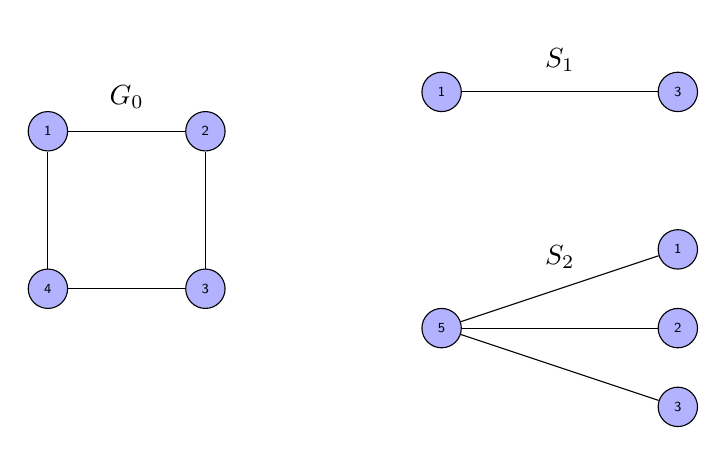
\begin{tikzpicture}[ node distance=1cm, every node/.style={base}, align=center, tight background]
                
                \tikzset{node distance = 2cm}
                \node (g01) at (-1,0.5){1};
                \node[right of=g01] (g02)  {2};
                \node[below of=g02] (g03)  {3};
                \node[below of=g01] (g04)  {4};
                \draw (g01) -- (g02) node [label, midway, above] {$G_0$};
                \draw (g02) -- (g03);
                \draw (g03) -- (g04);
                \draw (g04) -- (g01);
                \tikzset{node distance = 1cm}

                
                \node(s11) at (4,1){1};
                \node(s13) at (7,1){3};
                \draw (s11) -- (s13) node [label, midway, above] {$S_1$};

                \node(s25) at (4, -2) {5};
                \node[right of=s25, xshift=2cm](s22) {2};
                \node[above of=s22](s21) {1};
                \node[below of=s22](s23) {3};
                \draw (s25) -- (s21) node [label, midway, above] {$S_2$};
                \draw (s25) -- (s22);
                \draw (s25) -- (s23);

            \end{tikzpicture} 
    }
    \frame 
    {
    
        \frametitle{DMP Planarity Algorithm}
        \centering
            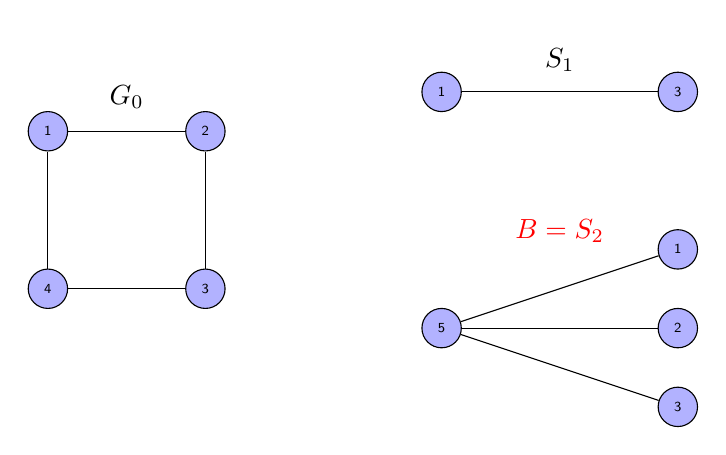
\begin{tikzpicture}[ node distance=1cm, every node/.style={base}, align=center, tight background]
                
                \tikzset{node distance = 2cm}
                \node (g01) at (-1,0.5){1};
                \node[right of=g01] (g02)  {2};
                \node[below of=g02] (g03)  {3};
                \node[below of=g01] (g04)  {4};
                \draw (g01) -- (g02) node [label, midway, above] {$G_0$};
                \draw (g02) -- (g03);
                \draw (g03) -- (g04);
                \draw (g04) -- (g01);
                \tikzset{node distance = 1cm}

                
                \node(s11) at (4,1){1};
                \node(s13) at (7,1){3};
                \draw (s11) -- (s13) node [label, midway, above] {$S_1$};

                \node(s25) at (4, -2) {5};
                \node[right of=s25, xshift=2cm](s22) {2};
                \node[above of=s22](s21) {1};
                \node[below of=s22](s23) {3};
                \draw (s25) -- (s21) node [label, midway, above, text=red] {$B =
                S_2$};
                \draw (s25) -- (s22);
                \draw (s25) -- (s23);

            \end{tikzpicture} 
    }

    \frame
    {
        \frametitle{DMP Planarity Algorithm}
        \begin{figure}
            \centering
            \SetCustomAlgoRuledWidth{5.5cm}
            \tiny
            \begin{subfigure}[h]{5.5cm} 
                \begin{algorithm}[H]
                    \NoCaptionOfAlgo
                    \DontPrintSemicolon
                    \KwInput{A 2-connected graph G}
                    \KwOutput{A planar embedding or FALSE}
                        $G_0$ := any cycle in G \;
                        
                        \While{$G_j \neq G$}
                        {
                            \If{any segment is blocked}
                            {
                                \Return FALSE \;
                            }
                            \If{a segment is forced}
                            {
                                $B :=$ that segment \;
                            }
                            \Else
                            {
                                $B :=$ any segment \;
                            }
                            $r :=$ region whose boundary contacts $B$ \;
                        }
                    
                    \caption{\tiny DMP Algorithm}
                \end{algorithm}
            \end{subfigure}
        \end{figure}
        \vfill
    }

    \frame 
    {
    
        \frametitle{DMP Planarity Algorithm}
        \centering
            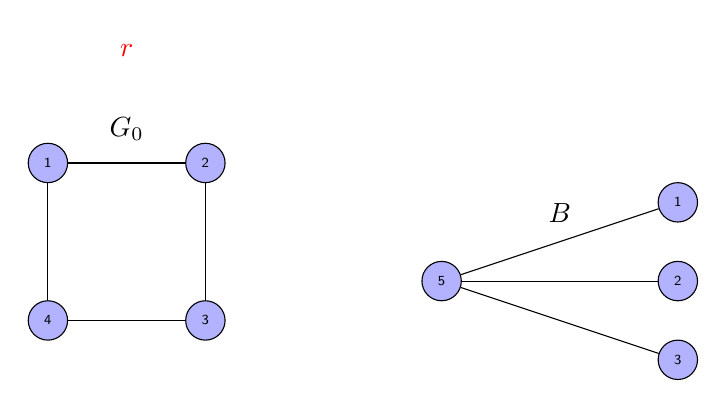
\begin{tikzpicture}[ node distance=1cm, every node/.style={base}, align=center, tight background]
                
                \tikzset{node distance = 2cm}
                \node (g01) at (-1,0.5){1};
                \node[right of=g01] (g02)  {2};
                \node[below of=g02] (g03)  {3};
                \node[below of=g01] (g04)  {4};
                \draw (g01) -- (g02) node [label, midway, above] (g0) {$G_0$};
                \draw (g02) -- (g03);
                \draw (g03) -- (g04);
                \draw (g04) -- (g01);
                \tikzset{node distance = 1cm}


                \node(s25) at (4, -1) {5};
                \node[right of=s25, xshift=2cm](s22) {2};
                \node[above of=s22](s21) {1};
                \node[below of=s22](s23) {3};
                \draw (s25) -- (s21) node [label, midway, above] {$B$};
                \draw (s25) -- (s22);
                \draw (s25) -- (s23);
                
                \pause
                \node[label, text=red, above of=g0] {$r$};
            \end{tikzpicture} 
    }

    \frame
    {
        \frametitle{DMP Planarity Algorithm}
        \begin{figure}
            \centering
            \SetCustomAlgoRuledWidth{5.5cm}
            \tiny
            \begin{subfigure}[h]{5.5cm} 
                \begin{algorithm}[H]
                    \NoCaptionOfAlgo
                    \DontPrintSemicolon
                    \KwInput{A 2-connected graph G}
                    \KwOutput{A planar embedding or FALSE}
                        $G_0$ := any cycle in G \;
                        
                        \While{$G_j \neq G$}
                        {
                            \If{any segment is blocked}
                            {
                                \Return FALSE \;
                            }
                            \If{a segment is forced}
                            {
                                $B :=$ that segment \;
                            }
                            \Else
                            {
                                $B :=$ any segment \;
                            }
                            $r :=$ region whose boundary contacts $B$ \;
                            $P :=$ path between two contact points of $B$ \;
                        }
                    
                    \caption{\tiny DMP Algorithm}
                \end{algorithm}
            \end{subfigure}
        \end{figure}
        \vfill
    }
    
    \frame 
    {
    
        \frametitle{DMP Planarity Algorithm}
        \centering
            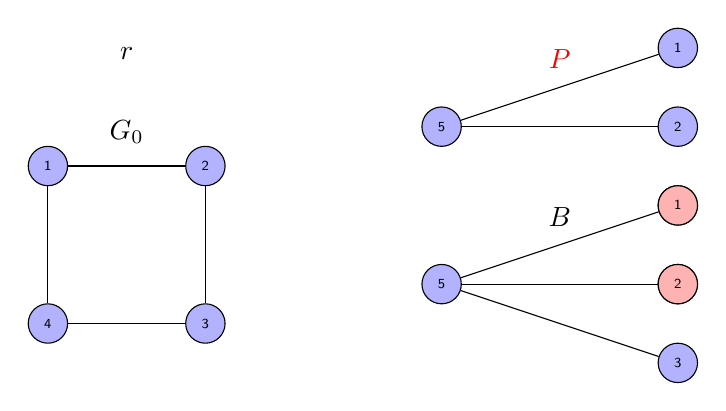
\begin{tikzpicture}[ node distance=1cm, every node/.style={base}, align=center, tight background]
                
                \tikzset{node distance = 2cm}
                \node (g01) at (-1,0.5){1};
                \node[right of=g01] (g02)  {2};
                \node[below of=g02] (g03)  {3};
                \node[below of=g01] (g04)  {4};
                \draw (g01) -- (g02) node [label, midway, above] (g0) {$G_0$};
                \draw (g02) -- (g03);
                \draw (g03) -- (g04);
                \draw (g04) -- (g01);
                \tikzset{node distance = 1cm}


                \node(s25) at (4, -1) {5};
                \node[right of=s25, xshift=2cm](s22) {2};
                \node[above of=s22](s21) {1};
                \node[below of=s22](s23) {3};
                \draw (s25) -- (s21) node [label, midway, above] {$B$};
                \draw (s25) -- (s22);
                \draw (s25) -- (s23);
                
                \node[label, above of=g0] {$r$};

                \pause
                \node[above of=s22, fill=red!30](s21red) {1};
                \node[right of=s25, xshift=2cm, fill=red!30](s22red) {2};
                
                \pause
                \node(p5) at (4, 1) {5};
                \node[right of=p5, xshift=2cm](p2) {2};
                \node[above of=p2](p1) {1};
                \draw (p5) -- (p1) node [label, midway, above, text=red] {$P$};
                \draw (p5) -- (p2);
            \end{tikzpicture} 
    }

    \frame
    {
        \frametitle{DMP Planarity Algorithm}
        \begin{figure}
            \centering
            \SetCustomAlgoRuledWidth{5.5cm}
            \tiny
            \begin{subfigure}[h]{5.5cm} 
                \begin{algorithm}[H]
                    \NoCaptionOfAlgo
                    \DontPrintSemicolon
                    \KwInput{A 2-connected graph G}
                    \KwOutput{A planar embedding or FALSE}
                        $G_0$ := any cycle in G \;
                        
                        \While{$G_j \neq G$}
                        {
                            \If{any segment is blocked}
                            {
                                \Return FALSE \;
                            }
                            \If{a segment is forced}
                            {
                                $B :=$ that segment \;
                            }
                            \Else
                            {
                                $B :=$ any segment \;
                            }
                            $r :=$ region whose boundary contacts $B$ \;
                            $P :=$ path between two contact points of $B$ \;
                            $G_{j+1} :=$ drawing of $P$ in $r$ \;
                        }
                    
                    \caption{\tiny DMP Algorithm}
                \end{algorithm}
            \end{subfigure}
        \end{figure}
        \vfill
    }
    
    \frame 
    {
    
        \frametitle{DMP Planarity Algorithm}
        \centering
            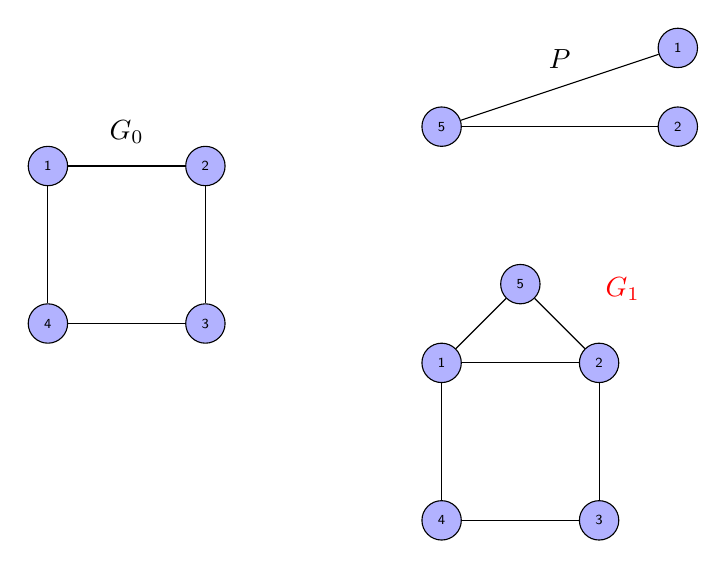
\begin{tikzpicture}[ node distance=1cm, every node/.style={base}, align=center, tight background]
                
                \tikzset{node distance = 2cm}
                \node (g01) at (-1,0.5){1};
                \node[right of=g01] (g02)  {2};
                \node[below of=g02] (g03)  {3};
                \node[below of=g01] (g04)  {4};
                \draw (g01) -- (g02) node [label, midway, above] (g0) {$G_0$};
                \draw (g02) -- (g03);
                \draw (g03) -- (g04);
                \draw (g04) -- (g01);
                \tikzset{node distance = 1cm}

                \node(p5) at (4, 1) {5};
                \node[right of=p5, xshift=2cm](p2) {2};
                \node[above of=p2](p1) {1};
                \draw (p5) -- (p1) node [label, midway, above] {$P$};
                \draw (p5) -- (p2);
                \pause

                \tikzset{node distance = 2cm}
                \node (g11) at (4,-2){1};
                \node[right of=g11] (g12)  {2};
                \node[below of=g12] (g13)  {3};
                \node[below of=g11] (g14)  {4};
                \node[above of=g11, xshift=1cm, yshift=-1cm] (g15)  {5};
                \draw (g11) -- (g12) ;
                \draw (g12) -- (g13);
                \draw (g13) -- (g14);
                \draw (g14) -- (g11);
                \draw (g11) -- (g15);
                \draw (g12) -- (g15) node [label, midway, above, text=red, xshift=0.8cm] (g0) {$G_1$};
                \tikzset{node distance = 1cm}
            \end{tikzpicture} 
    }

    \frame 
    {
    
        \frametitle{DMP Planarity Algorithm}
        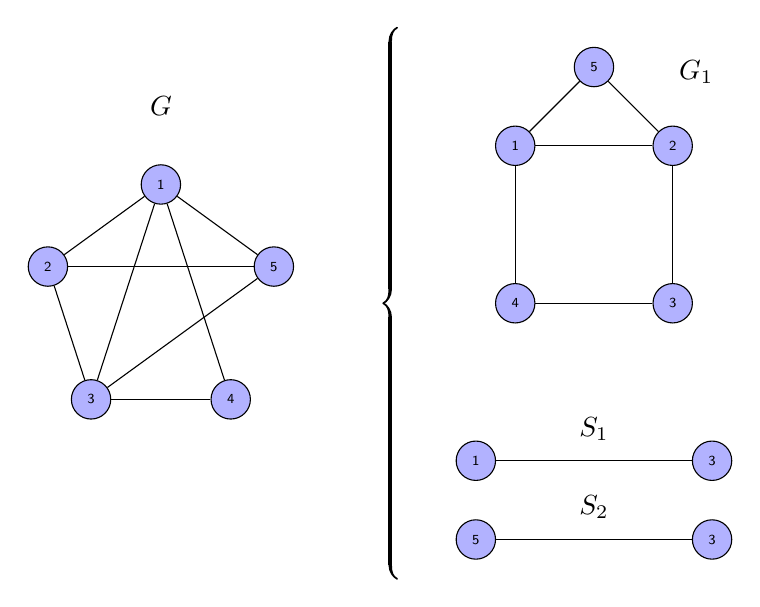
\begin{tikzpicture}[ node distance=1cm, every node/.style={base}, align=center, tight background]
            \def\ngon{5}
            \node[color=white, regular polygon,regular polygon sides=\ngon,minimum size=3cm] (p) {};
            \foreach\x in {1,...,\ngon}{\node (p\x) at (p.corner \x){\tiny \x};}
            \foreach\x in {1,...,\numexpr\ngon-2\relax}{
                \foreach\y in {\number\numexpr\x+1\relax}{\draw (p\x) -- (p\y);}
            }
            \draw (p1) -- (p3);
            \draw (p1) -- (p4);
            \draw (p1) --(p5);
            \draw (p2) -- (p5);
            \draw (p3) -- (p5);
            
            
            \draw[decorate, decoration={calligraphic brace,amplitude=5pt}, line
            width=1.25pt] (3,-3.5) -- (3,3.5);
            \node[label, above of=p1]{$G$};

            \tikzset{node distance = 2cm}
            \node (g11) at (4.5,2){1};
            \node[right of=g11] (g12)  {2};
            \node[below of=g12] (g13)  {3};
            \node[below of=g11] (g14)  {4};
            \node[above of=g11, xshift=1cm, yshift=-1cm] (g15)  {5};
            \draw (g11) -- (g12) ;
            \draw (g12) -- (g13);
            \draw (g13) -- (g14);
            \draw (g14) -- (g11);
            \draw (g11) -- (g15);
            \draw (g12) -- (g15) node [label, midway, above, xshift=0.8cm] (g0) {$G_1$};
            \tikzset{node distance = 1cm}
            \pause

            
            \node(s11) at (4,-2){1};
            \node(s13) at (7,-2){3};
            \draw (s11) -- (s13) node [label, midway, above] {$S_1$};
            \pause

            \node[below of=s11](s25) {5};
            \node[right of=s25, xshift=2cm](s23) {3};
            \draw (s25) -- (s23) node [label, midway, above] {$S_2$};
        \end{tikzpicture} 

    }
    
    \frame
    {
        \frametitle{DMP Planarity Algorithm}
        \begin{figure}
            \centering
            \SetCustomAlgoRuledWidth{5.5cm}
            \tiny
            \begin{subfigure}[h]{5.5cm} 
                \begin{algorithm}[H]
                    \NoCaptionOfAlgo
                    \DontPrintSemicolon
                    \KwInput{A 2-connected graph G}
                    \KwOutput{A planar embedding or FALSE}
                        $G_0$ := any cycle in G \;
                        
                        \While{$G_j \neq G$}
                        {
                            \If{any segment is blocked}
                            {
                                \Return FALSE \;
                            }
                            \If{a segment is forced}
                            {
                                $B :=$ that segment \;
                            }
                            \Else
                            {
                                $B :=$ any segment \;
                            }
                            $r :=$ region whose boundary contacts $B$ \;
                            $P :=$ path between two contact points of $B$ \;
                            $G_{j+1} :=$ drawing of $P$ in $r$ \;
                        }
                    
                    \caption{\tiny DMP Algorithm}
                \end{algorithm}
            \end{subfigure}
        \end{figure}
        \vfill
    }
    
    \frame 
    {
    
        \frametitle{DMP Planarity Algorithm}
        \centering
            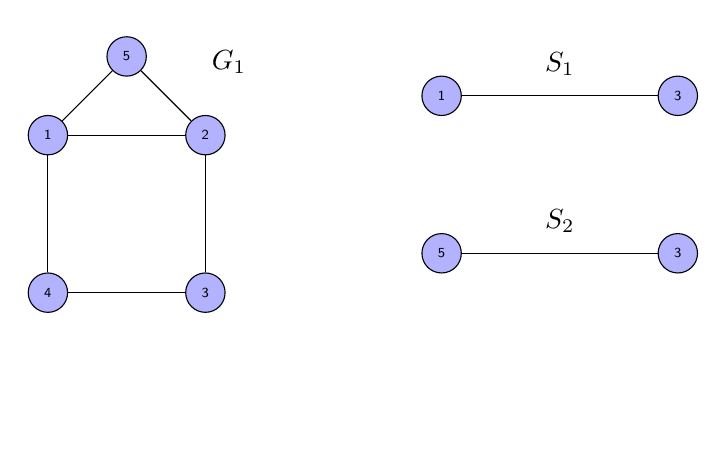
\begin{tikzpicture}[ node distance=1cm, every node/.style={base}, align=center, tight background]
                
                \tikzset{node distance = 2cm}
                \node (g11) at (-1,0.5){1};
                \node[right of=g11] (g12)  {2};
                \node[below of=g12] (g13)  {3};
                \node[below of=g11] (g14)  {4};
                \node[above of=g11, xshift=1cm, yshift=-1cm] (g15)  {5};
                \draw (g11) -- (g12) ;
                \draw (g12) -- (g13);
                \draw (g13) -- (g14);
                \draw (g14) -- (g11);
                \draw (g11) -- (g15);
                \draw (g12) -- (g15) node [label, midway, above, xshift=0.8cm] (g1) {$G_1$};
                \tikzset{node distance = 1cm}
                

                \node(s11) at (4,1){1};
                \node(s13) at (7,1){3};
                \draw (s11) -- (s13) node [label, midway, above] {$S_1$};

                \node[below of=s11, yshift=-1cm](s25) {5};
                \node[right of=s25, xshift=2cm](s23) {3};
                \draw (s25) -- (s23) node [label, midway, above] {$S_2$};

                \tikzset{every node/.style={opacity=0}}
                \node[below of=s25, yshift=-1cm](p5) {5};
                \node[right of=p5, xshift=2cm](p3) {3};
                
                \node[right of=g1] (r) {$r$};

            \end{tikzpicture} 
            \vfill
    }

    \frame 
    {
    
        \frametitle{DMP Planarity Algorithm}
        \centering
            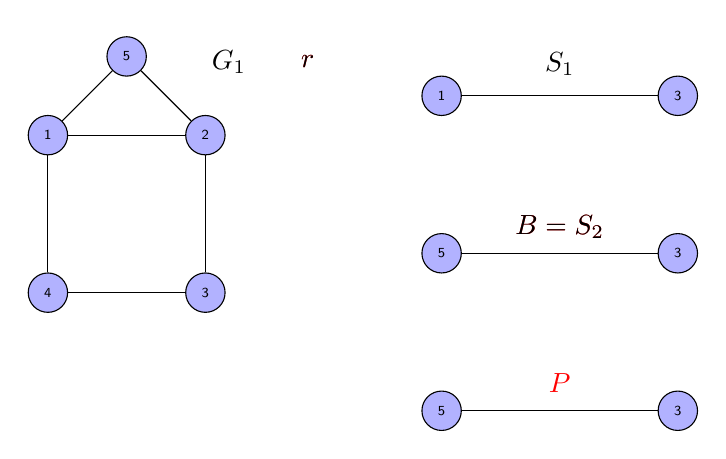
\begin{tikzpicture}[ node distance=1cm, every node/.style={base}, align=center, tight background]
                
                \tikzset{node distance = 2cm}
                \node (g11) at (-1,0.5){1};
                \node[right of=g11] (g12)  {2};
                \node[below of=g12] (g13)  {3};
                \node[below of=g11] (g14)  {4};
                \node[above of=g11, xshift=1cm, yshift=-1cm] (g15)  {5};
                \draw (g11) -- (g12) ;
                \draw (g12) -- (g13);
                \draw (g13) -- (g14);
                \draw (g14) -- (g11);
                \draw (g11) -- (g15);
                \draw (g12) -- (g15) node [label, midway, above, xshift=0.8cm] (g1) {$G_1$};
                \tikzset{node distance = 1cm}
                

                \node(s11) at (4,1){1};
                \node(s13) at (7,1){3};
                \draw (s11) -- (s13) node [label, midway, above] {$S_1$};

                \node[below of=s11, yshift=-1cm](s25) {5};
                \node[right of=s25, xshift=2cm](s23) {3};
                \draw (s25) -- (s23) node (redthing) [label, midway, above, text=red, yshift=-0.4cm]
                {$B=S_2$};
                
                \pause
                \node[label, text=red, right of=g1] (r) {$r$};
                \node[label, above of=redthing, yshift = -1cm, text=black] {$B=S_2$};
                \pause
                \node[below of=s25, yshift=-1cm](p5) {5};
                \node[right of=p5, xshift=2cm](p3) {3};
                \draw (p5) -- (p3) node [label, midway, above, text=red] {$P$};
                \node[label, text=black, right of=g1] (r) {$r$};
                
                
            \end{tikzpicture} 
            \vfill
    }

    \frame 
    {
    
        \frametitle{DMP Planarity Algorithm}
        \centering
            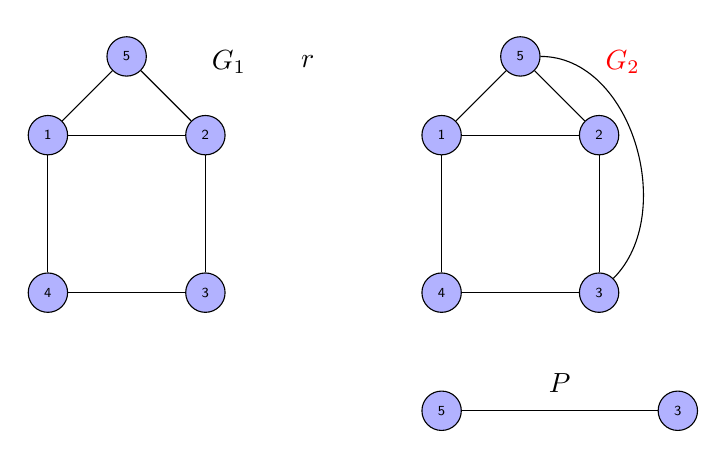
\begin{tikzpicture}[ node distance=1cm, every node/.style={base}, align=center, tight background]
                
                \tikzset{node distance = 2cm}
                \node (g11) at (-1,0.5){1};
                \node[right of=g11] (g12)  {2};
                \node[below of=g12] (g13)  {3};
                \node[below of=g11] (g14)  {4};
                \node[above of=g11, xshift=1cm, yshift=-1cm] (g15)  {5};
                \draw (g11) -- (g12) ;
                \draw (g12) -- (g13);
                \draw (g13) -- (g14);
                \draw (g14) -- (g11);
                \draw (g11) -- (g15);
                \draw (g12) -- (g15) node [label, midway, above, xshift=0.8cm] (g1) {$G_1$};
                \tikzset{node distance = 1cm}
                
                \node[label, right of=g1] (r) {$r$};
                
                \node[ yshift=-1cm](p5) at (4,-2) {5};
                \node[right of=p5, xshift=2cm](p3) {3};
                \draw (p5) -- (p3) node [label, midway, above] {$P$};
                \pause

                \tikzset{node distance = 2cm}
                \node[right of=g12, xshift=1cm] (g21) {1};
                \node[right of=g21] (g22)  {2};
                \node[below of=g22] (g23)  {3};
                \node[below of=g21] (g24)  {4};
                \node[above of=g21, xshift=1cm, yshift=-1cm] (g25)  {5};
                \draw (g21) -- (g22) ;
                \draw (g22) -- (g23);
                \draw (g23) -- (g24);
                \draw (g24) -- (g21);
                \draw (g21) -- (g25);
                \draw (g25) to[in=45, out=0] (g23);
                \draw (g22) -- (g25) node [label, midway, above, xshift=0.8cm, text=red] (g2) {$G_2$};
                \tikzset{node distance = 1cm}
                
            \end{tikzpicture} 
            \vfill
    }

    \frame 
    {
    
        \frametitle{DMP Planarity Algorithm}
        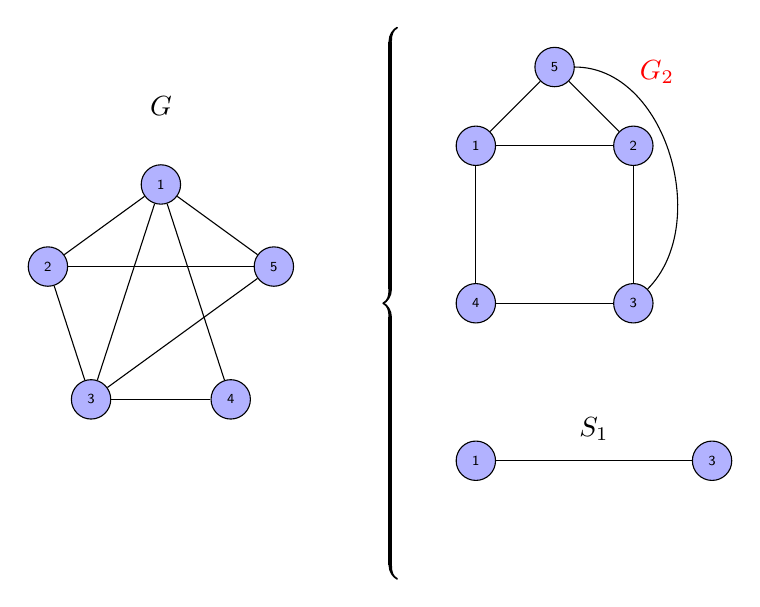
\begin{tikzpicture}[ node distance=1cm, every node/.style={base}, align=center, tight background]
            \def\ngon{5}
            \node[color=white, regular polygon,regular polygon sides=\ngon,minimum size=3cm] (p) {};
            \foreach\x in {1,...,\ngon}{\node (p\x) at (p.corner \x){\tiny \x};}
            \foreach\x in {1,...,\numexpr\ngon-2\relax}{
                \foreach\y in {\number\numexpr\x+1\relax}{\draw (p\x) -- (p\y);}
            }
            \draw (p1) -- (p3);
            \draw (p1) -- (p4);
            \draw (p1) --(p5);
            \draw (p2) -- (p5);
            \draw (p3) -- (p5);
            
            
            \draw[decorate, decoration={calligraphic brace,amplitude=5pt}, line
            width=1.25pt] (3,-3.5) -- (3,3.5);
            \node[label, above of=p1]{$G$};

            \tikzset{node distance = 2cm}
            \node (g21) at (4,2) {1};
            \node[right of=g21] (g22)  {2};
            \node[below of=g22] (g23)  {3};
            \node[below of=g21] (g24)  {4};
            \node[above of=g21, xshift=1cm, yshift=-1cm] (g25)  {5};
            \draw (g21) -- (g22) ;
            \draw (g22) -- (g23);
            \draw (g23) -- (g24);
            \draw (g24) -- (g21);
            \draw (g21) -- (g25);
            \draw (g25) to[in=45, out=0] (g23);
            \draw (g22) -- (g25) node [label, midway, above, xshift=0.8cm, text=red] (g2) {$G_2$};
            \tikzset{node distance = 1cm}
            \pause

            
            \node(s11) at (4,-2){1};
            \node(s13) at (7,-2){3};
            \draw (s11) -- (s13) node [label, midway, above] {$S_1$};
        \end{tikzpicture} 

    }

    \frame 
    {
    
        \frametitle{DMP Planarity Algorithm}
        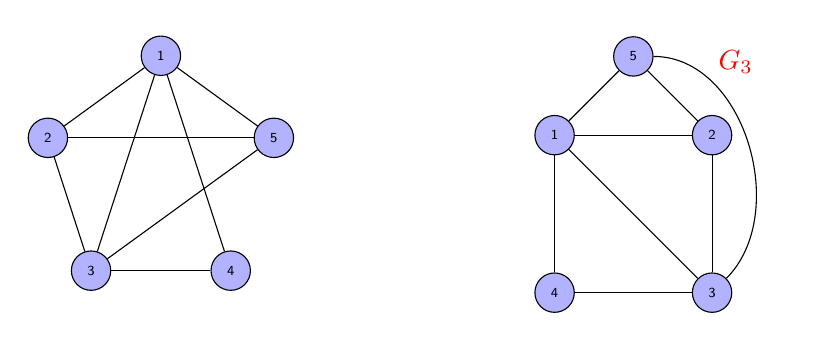
\begin{tikzpicture}[ node distance=1cm, every node/.style={base}, align=center, tight background]
            
            \tikzset{node distance = 2cm}
            \node (g21) at (5,.5) {1};
            \node[right of=g21] (g22)  {2};
            \node[below of=g22] (g23)  {3};
            \node[below of=g21] (g24)  {4};
            \node[above of=g21, xshift=1cm, yshift=-1cm] (g25)  {5};
            \draw (g21) -- (g22) ;
            \draw (g22) -- (g23);
            \draw (g23) -- (g24);
            \draw (g24) -- (g21);
            \draw (g21) -- (g25);
            \draw (g21) -- (g23);
            \draw (g25) to[in=45, out=0] (g23);
            \draw (g22) -- (g25) node [label, midway, above, xshift=0.8cm, text=red] (g2) {$G_3$};
            \tikzset{node distance = 1cm}
            
            \pause
            \def\ngon{5}
            \node[color=white, regular polygon,regular polygon sides=\ngon,minimum size=3cm] (p) {};
            \foreach\x in {1,...,\ngon}{\node (p\x) at (p.corner \x){\tiny \x};}
            \foreach\x in {1,...,\numexpr\ngon-2\relax}{
                \foreach\y in {\number\numexpr\x+1\relax}{\draw (p\x) -- (p\y);}
            }
            \draw (p1) -- (p3);
            \draw (p1) -- (p4);
            \draw (p1) --(p5);
            \draw (p2) -- (p5);
            \draw (p3) -- (p5);
        \end{tikzpicture} 

    }

    \frame
    {
        \frametitle{DMP Planarity Algorithm}
        \begin{figure}
            \centering
            \SetCustomAlgoRuledWidth{5.5cm}
            \tiny
            \begin{subfigure}[h]{5.5cm} 
                \begin{algorithm}[H]
                    \NoCaptionOfAlgo
                    \DontPrintSemicolon
                    \KwInput{A 2-connected graph G}
                    \KwOutput{A planar embedding or FALSE}
                        $G_0$ := any cycle in G \;
                        
                        \While{$G_j \neq G$}
                        {
                            \If{any segment is blocked}
                            {
                                \Return FALSE \;
                            }
                            \If{a segment is forced}
                            {
                                $B :=$ that segment \;
                            }
                            \Else
                            {
                                $B :=$ any segment \;
                            }
                            $r :=$ region whose boundary contacts $B$ \;
                            $P :=$ path between two contact points of $B$ \;
                            $G_{j+1} :=$ drawing of $P$ in $r$ \;
                        }
                    \Return{$G_j$}
                    \caption{\tiny DMP Algorithm}
                \end{algorithm}
            \end{subfigure}
        \end{figure}
        \vfill
    }
    
    \section{Other Surfaces?}

    \frame
    {
    \frametitle{What about other surfaces?}
        \textbf{Sphere?} \pause same as plane

        \medskip
        \textbf{Annulus?} \pause same as plane
        
        \medskip
        \textbf{Torus?} \pause different!

        \bigskip
        
    }
\end{document}
    